
\documentclass[bsc,frontabs,singlespacing,parskip]{infthesis} % add [twoside]
\usepackage{filecontents}
\usepackage{fancyvrb}
\usepackage{graphicx}
\usepackage[export]{adjustbox}

\begin{document}
\long\def\/*#1*/{}

\title{Representing Films as Character Graphs}

\author{Victor Dumitrescu}

\course{Artificial Intelligence and Computer Science}
\project{4th Year Project Report (Interim)}

\date{\today}

\abstract{
This project sets out to explore a representation of films in terms of their characters, based on textual information, such as screenplays and plot summaries. The work described in this report builds upon the existing literature in computational linguistics concerned with studying characters in films and other works of fiction. The character graphs presented here model two main aspects of film characters: their personalities and their role in the social network of the narrative. We try to show that by combining these two approaches in a single representation, we can derive some insight into establishing the similarity of films.
}

\maketitle

% \section*{Acknowledgements}
% Acknowledgements go here. 

%\tableofcontents

%\pagenumbering{arabic}  <-- was commented out in the skeleton too


\chapter{Work done so far}

\section{Background work}
Interest in computationally analysing narrative fiction has spiked along with the increasing number of raw data available to researchers. In order to establish the basis of the work described in this report, we will highlight some of the previous literature which atakes a character-centric point of view when approaching narrative fiction.

Recent work by David Bamman and others has explored the idea of learning the type or \textit{persona} of film \cite{Bamman2013} and literary \cite{Bamman2014} characters. A character persona is a probabilistic model of a character's personality traits, constructed using certain keywords from a film's plot summary. The papers present a number of variations of this model, but we will only describe the \textit{Dirichlet Persona Model}, which serves as the basis for our work.



\section{Data sets}
Three main sources of data used in this project are:
\begin{itemize}
	\item \textbf{CMU Movie Summary Corpus}, a collection of 42,306 Wikipedia plot summaries of films, along with metadata extracted from Freebase. The summaries are processed using the \textit{Stanford CoreNLP} tools, specifically tagging, parsing, named entity recognition and coreference resolution.
	\item \textbf{ScriptBase} \cite{Gorinski}, a corpus of 1,276 film scripts, along with IMDB and Wikipedia metadata, similarly processed using \textit{Stanford CoreNLP} pipeline.
	\item \textbf{Rotten Tomatoes} film similarity data, collected through their official API. It comprises of pairs of similar films, reflecting human judgements.
\end{itemize}

The first two corpora are used to construct the character graphs. The Rotten Tomatoes data provides the basis for a gold-standard measure of film similarity, which we use to assess the usefulness of the character graph representations.

\section{The processing pipeline}
This section details the components of the pipeline constructed as part of the project to acquire and process data, construct character graphs, compare them and assess the results.

\subsection{The Character Graph}
In order to construct the character graph for a film we need to find a meaningful representation of the relationship between characters (the nodes in our graph). For simplicity, we can start by trying to find a numerical measure, which would correspond to edge weights in an undirected weighted graph. The measure we have used in this project is the number of scene co-occurrences between two characters. Thus, the weight of an edge between two characters represents the number of scenes in which those characters appear together. When comparing the character graphs of different films, these weights will be normalised (by the total number of scenes in the film).

Apart from simplicity, choosing this measure can enable us to reliably discover the main characters of a film using a graph centrality indicator. However, scene co-occurrence does not give any insights into the \textit{nature} of the interaction between characters.

\subsubsection{Processing ScriptBase screenplays}
To ease the task of extracting the number of character to character scene co-occurrences, we restricted the set of films to the 127 which have already been processed in ScriptBase. A processed script is an XML file which, apart from the standard CoreNLP annotations, also places every sentence inside a numbered \texttt{scene} tag. It also distinguishes between stage directions and speech, annotating the name of the speaker(s) in the latter case.

Thus, it is straightforward to parse the XML document and, for each pair of characters, record the number of scenes in which they both have at least one line of speech. Note that although this approach ignores characters which might be present in a scene but do not speak, in practice we do not expect this to influence the results significantly.

\subsubsection{Constructing character graphs}
For representing character graphs, we have chosen GEXF \footnote{The GEXF file format, \textit{http://gexf.net}}, a standard XML format for describing general network structures. As described above, we simply extract all the character names from the script and use them as the set of nodes in the graph. We add a weighted edge for all the recorded interactions between characters. As a result, every film (of the 127 which we considered) will be represented with a GEXF file.

\begin{figure}
	\centering
	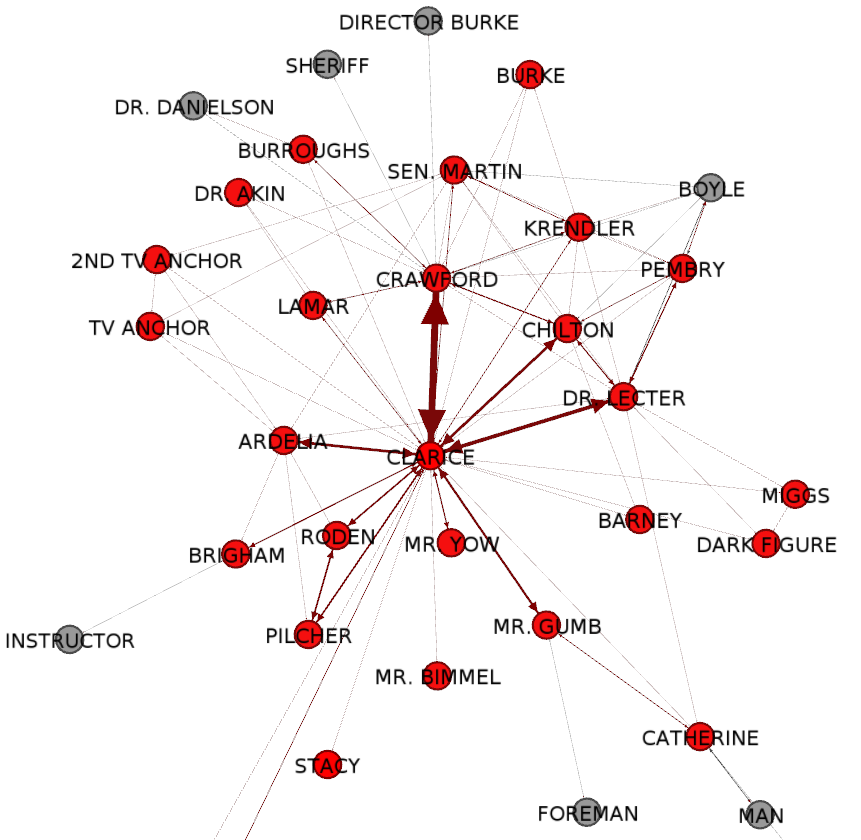
\includegraphics[scale=0.4]{clarice_graph}
	\caption{Character graph of \textit{The Silence of the Lambs} (1991), centered around the protagonist, Clarice Starling. Edge size is proportional to the number of scene co-occurrences between two characters.}
\end{figure}

\subsection{The Persona Model}
We implemented a variation of the Dirichlet Persona Model introduced in \cite{Bamman2013} and briefly described above.
\subsubsection{Processing the CMU script summaries}
The CMU corpus provides both the raw plot summaries and a file containing all the processed summaries, which can be used as input for the pipeline described in their paper. We have designed ours to work with the same input format, enabling us to use the data from this corpus without any additional preprocessing, apart from filtering out the films for which we have not constructed a character graph. This includes the majority of films in the corpus. Out of the 127 films from ScriptBase, 96 also have a processed plot summary.

The filtered film data file contains, for each film and each character mentioned in the plot summary, a list of words which are either:
\begin{itemize}
	\item \textbf{Agent verbs:} Verbs for which the character is an agent (e.g. "Starling \textit{travels} to the victim's hometown")
	\item \textbf{Patient verbs:} Verbs for which the character is the patient or object (e.g. "Starling is \textit{led} to the house of Jack Gordon", where \textit{Starling} is a passive nominal subject)
	\item \textbf{Modifiers:} Other words which describe the characters (e.g. "Catherine is still \textit{alive}")
\end{itemize}

These words are selected into one of these types on the basis of their Stanford typed dependencies, as determined using the CoreNLP parser. Each of the three types described above corresponds to a list of dependencies and all tokens tagged with those dependencies will be assigned a type. In the final input file, in addition to the word lemma, its type (agent, patient, modifier) and its dependency tag, the word tuples for each character also contain the part of speech and the WordNet supersense.


\subsubsection{Constructing the persona model}
In this project we implement a simpler version of the Dirichlet persona model \cite{Blei2003}. The original model was implemented as generative model. In the paper, a persona is defined as a set of 3 distributions (corresponding to agent, patient and modifier words) over topics, which are in turn distributions over words, similar to topic in Latent Dirichlet Allocation.

We have opted to use the standard LDA algorithm, as implemented in the Python \texttt{lda 0.3.2} package \footnote{ www.pypi.python.org/pypi/lda} in order to derive the latent topics in our vocabulary and use a simple maximum likelihood estimation method to compute each character's 3 distributions over these latent topics.

One of the advantages of this frequentist approach is that the only parameter that we need to optimise in the model is the number of topics computed by the LDA algorithm. Since the number of films in our collection is small and largely restricted to two genres (thriller and comedy), we expect the number of meaningful topics to also be reasonably small. Therefore we have tried to manually vary this parameter and select the value which seems to intuitively give a complete coverage of topics, without having different topics which seem very close. We have used to highest probability words in each topic distribution as a guide. So far, we have settled on having 10 topics (\textit{Figure 1.2}).

\begin{figure}[h]
\centering
\begin{minipage}{8cm}
\begin{Verbatim}[frame=single]
0: tell take go have 
1: stop arrive hide officer 
2: mother decide love marry 
3: meet discover leave confront 
4: join wife know lie 
5: girl son offer husband 
6: give kill confront offer
7: kill shoot brother find 
8: pursue criminal escape ndapp
9: set capture try save 
\end{Verbatim}
\end{minipage}
\caption{First 4 words in the 10 topics discovered by LDA on our film collection, ranked by probability.}
\label{topics}
\end{figure}

Having these 10 distributions over words in the vocabulary, we construct, for each character, a set of 3 distributions over these topics, by multiplying the number of different occurrences of a certain word lemma with the probability of that lemma in a certain topic, then normalising. It is then easy to compare the persona of two different characters, by using any distance measure, such as Euclidean distance.

\subsection{Comparing character graphs}
Once the character graphs are constructed, the nodes can be annotated with the persona information. Note that although the character graphs are likely to contain a node for every character in the plot (a small variation can occur due to faults in the preprocessing of scripts), personas will be computed for 2-5 main characters. Again, due to the limitations of the standard NLP tools (most notably coreference resolution), this number can be lower, sometimes even 0.

To represent annotated graphs in our project, we have used the Python \texttt{networkx} library \footnote{www.networkx.github.io}.

\subsubsection{Direct matching based on centrality}
The simplest comparison measure implemented is based on matching characters from different graphs based on their role in the network. Using degree centrality, the nodes of each graph are sorted and only the first 10 nodes are kept. This is a parameter that can be experimentally adjusted, but we have set it to 10 initially because for every film in the collection, we could not compute a persona for any character that has rank below 10 by degree centrality.

Then, every pair of corresponding characters (by rank) in the two graphs is compared. Note that although a persona is a set of 3 distributions, not all characters will have a distribution defined for all 3 types (agent, patient, modifier), since the relevant word lemmas might not be present in the plot summary. Therefore, we compare the distributions which both characters have in common, by taking the norm of the difference between the 2 vectors. The film similarity score is computed as the average of these differences: the lower the score, the more similar the graphs are deemed to be.

\begin{figure}[h]
\centering
\begin{minipage}{11.5cm}
\begin{Verbatim}[frame=single]
Star Trek V    - The Anniversary Party     (0.00167)
Ghost World    - I Love You Phillip Morris (0.00193)
Ghost World    - Copycat                   (0.00202)
Ghost World    - Clerks                    (0.00236)
Ghost World    - Miller's Crossing         (0.00257)
Ghost World    - Nick of Time              (0.00275)
Ghost World    - Sweeney Todd              (0.00338)
The Informant! - The Hangover              (0.00351)
Ghost World    - Gothika                   (0.00352)
Jaws           - Living in Oblivion        (0.00410)
\end{Verbatim}
\end{minipage}
\caption{The 10 most similar pair of films in our collection of 96 thrillers and comedies, based on comparing personas matched by degree centrality rank}
\end{figure}

In these results, it is easy to see that the comedy \textit{Ghost World} dominates the similarity pairings, being matched both with comedies and thrillers. Overall, the results do not seem to be very revealing. To understand why this might be the case, let us explore the example of \textit{Ghost World}, by showing the top 10 characters and the top 3 topics for each character that has a persona defined. Each topic is described by the top 3 most probable words in that topic.

\begin{figure}[h]
\centering
\begin{minipage}{9cm}
\begin{Verbatim}[frame=single]
ENID 
REBECCA [ M(join wife know)
          M(pursue criminal escape)
          M(girl son offer) ]
SEYMOUR [ P(tell take go)
          A(tell take go)
          A(meet discover leave) ]
ROBERTA [ A(give kill confront)
          A(girl son offer)
          M(girl son offer) ]
JOE 
CUSTOMER 
PAUL 
GERROLD 
JEROME 
STEVEN 
\end{Verbatim}

\end{minipage}
\caption{The 10 most central characters in \textit{Ghost World} and their personas}
\end{figure}

One explanation for the dominance of \textit{Ghost World} in the similarity results shown above is the fact that its characters seem to be typical of both romantic comedies (topics such as \texttt{(join wife know)} or \texttt{(meet discover leave)}) and thrillers (topics like \texttt{(give kill confront)}).

We suspect that one of the causes of the weak results is the small number of films in our collection and, consequently, the small number of words in the vocabulary. This can lead to a topic clustering which does not have much discriminative power (see the list of topics in Figure \ref{topics}). It might also be the case that, since not many personas are matched between films, these occasional matches might be insufficient for obtaining meaningful results across the whole corpus.

\subsection{Rotten Tomatoes similarity}
One of the aims of the project is to determine whether character graphs can be useful in predicting film similarity, based on human judgements. Independent from the work described so far, we have also tried to construct a gold-standard collection of film similarity pairs, using data supplied by Rotten Tomatoes\footnote{www.rottentomatoes.com}. Their public API supports requests of the form "What films have users deemed to be similar to this one?" and offers up to 5 results.

We have found that the results obtained by querying every film in the collection and discarding every returned film which is not part of the collection yields a very small number of pairs. Thus, we have expanded the similarity measure by constructing a graph in which films are nodes and edges represent similarity and allowing films from outside the corpus. The similarity can then be measured as the minimum distance in the graph.

\subsection{Future work}
Over the next two weeks, I plan to:
\begin{itemize}

	\item parse more raw scripts from ScriptBase into processed XML files

	I have alredy started work on this, but the process is laborious because although scripts loosely follow the same format, the differences between them are quite substantial and make parsing difficult.

	\item explore different measures of film similarity
	
	Since relying on personas derived from plot summaries seems to be quite problematic, considering the small number of characters for which a persona can be estimated, I would like to explore other measures which rely more on the relationships between characters and the scripts. Some slightly more sophisticated ideas about this can be found in \cite{Gorinski}. If time allows, I could try an approach based on sentiment analysis, such as that described in \cite{Nalisnick2013}
	
	\item run experiment against the gold-standard film pairings
	
	Use the Rotten Tomatoes film similarity in order to assess the accuracy of the different methods I have been trying so far
\end{itemize}

\bibliographystyle{plain}
\bibliography{collection}

\end{document}
